

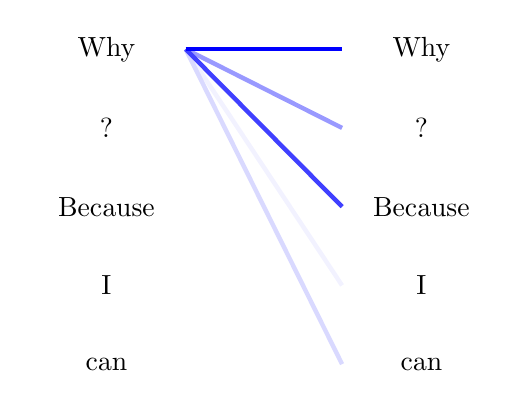
\begin{tikzpicture}[
    y=-1cm,
    every node/.style={minimum width=2cm},
]

    \node (why) at (0,0) {Why};
    \node (int) at (0,1) {?};
    \node (because) at (0,2) {Because};
    \node (i) at (0,3) {I};
    \node (can) at (0,4) {can};

    \node (why2) at (4,0) {Why};
    \node (int2) at (4,1) {?};
    \node (because2) at (4,2) {Because};
    \node (i2) at (4,3) {I};
    \node (can2) at (4,4) {can};

    \draw[-, draw=blue!5, ultra thick] (why.east) -- (i2.west);
    \draw[-, draw=blue!15, ultra thick] (why.east) -- (can2.west);
    \draw[-, draw=blue!40, ultra thick] (why.east) -- (int2.west);
    \draw[-, draw=blue!75, ultra thick] (why.east) -- (because2.west);
    \draw[-, draw=blue!100, ultra thick] (why.east) -- (why2.west);
\end{tikzpicture}
